Using the Classical PSHA-based or Probabilistic Event-based Calculators (\cite{SilvaEtAl2014a}, \cite{PaganiEtAl2014a}) of the OpenQuake-engine, it is possible to calculate seismic hazard curves for a number of locations, or loss exceedance curves considering a collection of spatially distributed assets.

\subsection{Plotting hazard curves and uniform hazard spectra}
\label{subsec:plot-hazard_curves}
A seismic hazard curve defines the probability of exceeding a number of intensity measure levels (e.g. peak ground acceleration or spectral acceleration) for a given interval of time (e.g. 50 years). In order to plot these curves, it is necessary to define the path to the output file in the parameter \verb=hazard_curve_file=. Then, since each output file might contained a great number of hazard curves, it is necessary to establish the location for each the hazard curve will be extracted. To visualize the list of locations comprised in the output file, the function \verb=hazard_curves.loc_list= can be employed. Then, the chosen location must be provided to the plotting function (e.g. \verb=hazard_curves.plot("81.213823|29.761172")=). An example of a seismic hazard curve is provided in Figure \ref{fig:hazard_curve}.\\

\begin{figure}[htb]
  \centering
      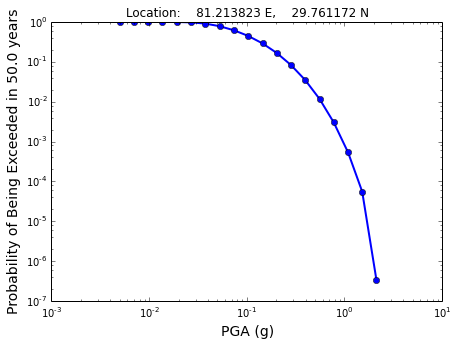
\includegraphics[width=9cm]{figures/hazard_curve.png}
  \caption{Seismic hazard curve for peak ground acceleration (PGA).}
  \label{fig:hazard_curve}
\end{figure}

To plot uniform hazard spectra (UHS), a similar approach should be followed. The output file containing the uniform hazard spectra should be defined using the parameter \verb=uhs_file=, and then a location must be provided to the plotting function (e.g.\verb=uhs.plot("81.213823|29.761172")=). An example of uniform hazard spectra is illustrated in Figure \ref{fig:UHS}.

\begin{figure}[htb]
  \centering
      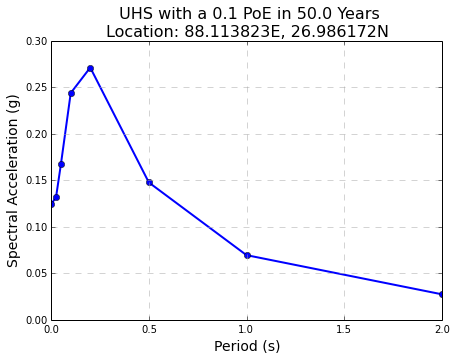
\includegraphics[width=9cm]{figures/UHS.png}
  \caption{Uniform Hazard Spectra for a probability of exceedance of 10\% in 50 years.}
  \label{fig:UHS}
\end{figure}

\subsection{Plotting loss curves}
\label{subsec:plot-loss_curves}
A loss exceedance curve defines the relation between a set of loss levels and the corresponding probability of exceedance within a given time span (e.g. a year). In order to plot these curves, it is necessary to define the location of the output file using the parameter \verb=loss_curves_file=. Since each output file may contains a large number of loss exceedance curves, it is necessary to define for which assets will the loss curves be extracted. The parameter \verb=assets_list= should be employed to define all of the chosen asset ids. These ids can be visualize directly on the loss curve output file, or on the exposure model used for the risk calculations. It is also possible to define a logarithmic scale for the x and y axis using the parameters \verb=log_scale_x= and \verb=log_scale_y=. A loss exceedance curve for a single asset is depicted in Figure \ref{fig:loss_curve}.

\begin{figure}[htb]
  \centering
      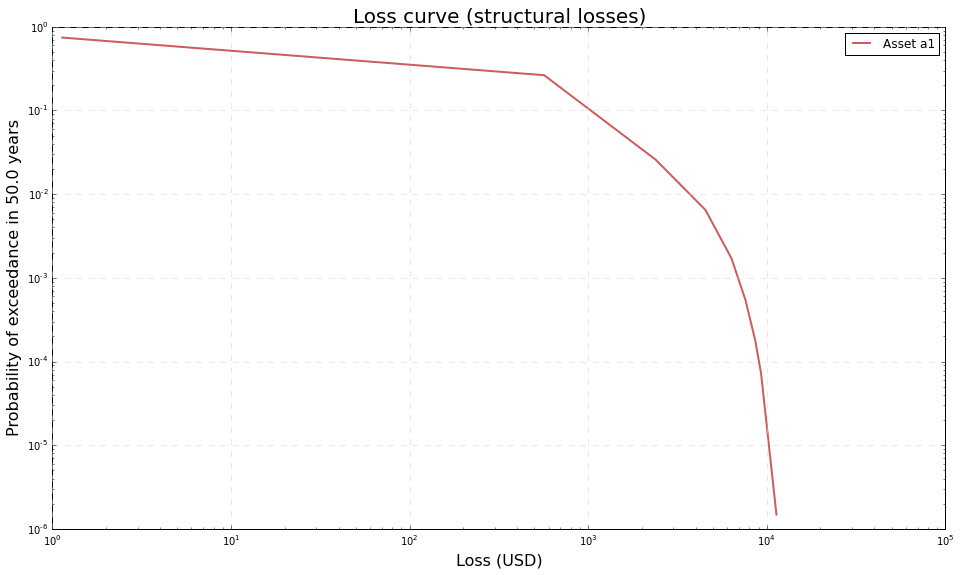
\includegraphics[width=8cm]{figures/loss_curve.png}
  \caption{Loss exceedance curve.}
  \label{fig:loss_curve}
\end{figure}